\documentclass[times, utf8, zavrsni]{fer}
\usepackage{booktabs}
\usepackage{graphicx}
\usepackage{array}
\usepackage{listings}
\usepackage{color}
\graphicspath{ {./img/} }

\begin{document}

% TODO: Navedite broj rada.
\thesisnumber{5417}

% TODO: Navedite naslov rada.
\title{Implementacija sustava za nadziranje i upravljanje bežičnim razvojnim modulima ESP8266}

% TODO: Navedite vaše ime i prezime.
\author{Ivan Trubić}

\maketitle

% Ispis stranice s napomenom o umetanju izvornika rada. Uklonite naredbu \izvornik ako želite izbaciti tu stranicu.
\izvornik

% Dodavanje zahvale ili prazne stranice. Ako ne želite dodati zahvalu, naredbu ostavite radi prazne stranice.
\zahvala{}

\tableofcontents

% Uvod {{{
\chapter{Uvod}
ESP8266 je System on Chip (SoC) rješenje tvrtke Espresiff Systems vrlo malene površine mnogih mogučnosti.
Dizajniran je kao vrlo jeftin modul sa mogučnošću spajanja na WiFi mrežu te niskom potrošnjom energije što ga čini vrlo povoljnim za ugrađivanje u IoT (\textit{Internet Of Things}) uređaje.
U ovome će radu ESP8266 \textit{SoC} biti korišten kao krajnji čvor u sustavu bežičnog prikupljanja podataka, nadziranja te upravljanja koji komunicira s ostalim sustavom koristeći \textit{Message Queueing Telemetry Transport} protokol (MQTT).
Topologija takvog sustava se sastoji od krajnjeg čvora na kojem je spojen neki uređaj koji želimo kontrolirati ili nadzirati, pristupne točke WiFi mreži, poslužitelja na kojemu se nalaze MQTT broker za upravljanje porukama, baza podataka koja sadrži trenutne podatke čvorova te API kao sučelje između baze podataka i krajnjeg klijenta.
Ovakav sustav je vrlo jednostavan i jeftin za implementaciju te je izrazito jako skalibilan što znači da pisanjem vrlo jednostavnog programskog koda za pojedini čvor možemo u svoju mrežu postaviti virtualno beskonačno krajnjih čvorova kojima se vrlo jednostavno može upravljati. 
Cilj ovoga rada je napraviti gotov sustav otvorenoga koda koji će prateći \textit{Homie} konvenciju za MQTT protokol olakšati amaterima brzo rađenje prototipa bilo iz znatiželje, potrebe ili kreativnosti.
%}}}

\chapter{Razrada}

% ESP {{{
\section{ESP8266}
ESP8266 je \textit{SoC} koji u sebi ima mikrokontroler RISC arhitekture te WiFi modul za spajanje na mrežu.
Ciljano tržište za ovaj čip su hobisti koji žele neku svoju ideju pretvoriti u stvarnost na vrlo jednostavan način.
Dizajniran je vrlo jednostavno i kompaktno kako bi cijena čipa bila što niža te zato što je namjenjen za jednostavne i lokalizirane poslove koji uključuju upravljanje vrlo malim brojem uređaja odjednom.
Točno u tome leži prava snaga čipa jer možemo imati više čipova koji komuniciraju međusobno umjesto da imamo jedan snažan mikrokontroler koji će upravljati uređajima centralizirano.

\begin{figure}[h]
    \centering
    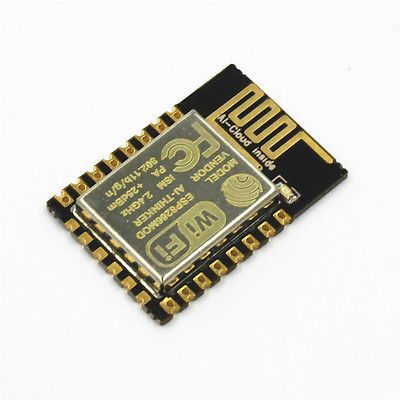
\includegraphics[scale=0.5]{esp8266.jpg}
    \caption{ESP8266 \textit{SoC}}
\end{figure}
%}}}

% Znacajke {{{
\section{Značajke}
ESP8266 u sebi ima 32-bitni RISC mikrokontroler koji radi na frekvenciji od 80MHz.
Memorija se sastoji od:
\begin{itemize}
    \item 32 KiB instrukcijskog RAM-a
    \item 32 KiB priručne memorije instrukcijskog RAM-a
    \item 80 KiB korisničkog RAM-a
\end{itemize}
Vanjske QSPI \textit{flash} memorije do 16MiB ovisno o modelu, IEEE 802.11 b/g/n WiFi, 16 GPIO pina, SPI sučelje, softverska implementacija I2C protokola, I2S sučelje, UART te 10-bitni analogno-digitalni pretvornik.
%}}}

% Povezivost {{{
\section{Povezivost}
Najbitnije sučelje prema vanjskome svijetu na ESP8266 su bežična mreža i 16 GPIO pinova.
Mreža podržava IEEE 802.11 b/g/n protokol, P2P konfiguraciju te TCP/IP protokolni stog.
GPIO pinovi se mogu zasebno programirati kao ulazi/izlazi, postaviti im \textit{pull-up/down} otpornike, te svaki ima ugrađen 10 bitni digitalno-analogni pretvornik tako da se svaki pin ponaša kao analogni izlaz.
Ima također jedan analogan ulaz sa 10 bitnim analogno-digitalnim pretvornikom za spajanje raznih analognih senzora bez posebnih sučelja.
%}}}

% Programiranje{{{
\section{Programiranje} 
ESP8266 se može programirati na više različitih načina.
Originalno se programirao uz pomoć drugoga mikrokontrolera sve dok firma Espressif Systems nije izdala poseban \textit{SDK}(  eng. \textit{Software Development Kit} ) nakon čega to više nije bilo potrebno.
Nakon toga su se počeli javljat mnogi SDK-ovi ponajviše otvorenog koda zajednice programera od čega su najpoznatiji:
    \begin{itemize}
        \item NodeMCU - baziran na skriptnom programskom jeziku Lua
        \item Arduino - baziran na jeziku C++ iste sintakse kao i bilokoji arduino mikrokontroler
        \item PlatformIO - nova razina razvoja ugradbenih sustava sa posebnim IDE-om
        \item MicroPython - baziran na programskom jeziku python
    \end{itemize}
%}}}

%Usporedba {{{
\section{Usporedba drugih razvojnih modula koji koriste WiFi komunikacijski protokol sa ESP8266 modulom}
Pronalazak alternativnih modula se pokazalo izazovno zbog tolike raširenosti ESP modula.
U tablici~\ref{tab:usporedba} je vidljivo i zašto je to tako.
Moduli CC3000 i RN-131 su u zajednici i od strane proizvođača označeni kao NRND (engl. \textit{Not Recommended for New Designs}) jer se više ne podržavaju.
Cijenovno niti funkcionalno nisu nimalo adekvatni za korištenje u \textit{IoT} svrhe.

%tablica {{{
\begin{center}
    \begin{table}[h]
        \begin{tabular}{ |c||c|c|c|c| }
            \hline
            \textbf{Kategorija} & \textbf{ESP8266} & \textbf{ESP32} & \textbf{CC3000} & \textbf{RN-131} \\
            \hline
            \hline
            \textbf{WiFi Standard} & 802.11 b/g/n & 802.11 b/g/n & 802.11 b/g & 802.11 b/g\\
            \hline
            \textbf{Tip paketa} & TCP i UDP & TCP i UDP & TCP i UDP & TCP i UDP\\
            \hline
            \textbf{Režim rada} & Klijent i Server & Klijent i Server & Klijent i Server & Klijent i Server\\
            \hline
            \textbf{AP režim} & P2P i Soft-AP & Soft-AP & Ne & Soft-AP\\
            \hline
            \textbf{Dimenzije [mm]} & 26x16x3 & 26x18x3 & 16.3x13.5x3 & 20x37x3.5\\
            \hline
            \textbf{Sučelje} & TTL-Serial & TTL-Serial & SPI & SPI\\
            \hline
            \textbf{Enkripcija} & WPA2-PSK & WPA2 i WAPI & WPA-PSK & WPA2-PSK\\
            \hline
            \textbf{Struja u sleep režimu rada} & <10 $\mu$A & 5 $\mu$A & ? & 4$\mu$A\\
            \hline
            \textbf{Struja napajanja} & 80mA & 500mA & ? & 40mA\\
            \hline
            \textbf{Napon napajanja} & 3.0-3.6V & 2.3-3.6V & 2.7-3.6V & 3.0-3.7\\
            \hline
            \textbf{Digitalni pinovi} & 9 & 34 & 0 & 10\\
            \hline
            \textbf{Analogni pinovi} & 1 & 18 & 0 & 8\\
            \hline
            \textbf{Sadrži mikrokontroler} & Da & Da & NE & Ne\\
            \hline
            \textbf{Cijena [\$]} & 6.95 & 8.95 & 34.95 & 35.38\\
            \hline
        \end{tabular}
        \caption{usporedba značajki WiFi modula i cjena}
        \label{tab:usporedba}
    \end{table}
\end{center}
%}}}

C3000 i RN-131 moduli nemaju programljivi mikrokontroler, ne koriste suvremeni 802.11n standard koji je znatno brži te su cjenovno i po nekoliko puta skuplji od vrlo močnih ESP modula.
Iz tog su se razloga ESP moduli probili na tržištu i u tolikoj se mjeri proširili.
%}}}

%MQTT {{{
\section{Message Queuing Telemetry Transport - \textbf{MQTT}}
MQTT je protokol široko primjenjen u \textit{IoT} sustavima temeljen na prijenosu poruka u režimu pretplate i objave.
Prijenos poruka se vrši preko TCP/IP protokola te se za to brine program na poslužitelju koji ima ulogu brokera.
Pretplata i objava se vrše na temelju teme (eng. \textit{topic}) gdje uređaji MQTT brokeru šalju poruke koje taj broker ovisno o temi šalje drugim uređajima koji su na tu temu pretplačeni.
Prava moć MQTT protokola su teme koje zamjenjuju MAC i IP adrese uređaja kako bi postavljanje infrastrukture postalo vrlo trivijalno i lagano za implementirati.
Tema je oblika \textit{"ovo/je/primjer/teme"} gdje je svaka razina teme odvojena separatorom \textit{"/"}.
Tema može imati bilokoliko razina te se one mogu adresirati pomoću zamjenskih znakova:
\begin{itemize}
    \item '+' - predstavlja jednu razinu u temi. Npr. tema \textit{"mojdom/prizemlje/+/temperatura"} će prikazivati sve poruke na temama \textit{"mojdom/prizemlje/kuhinja/temperatura"} te \textit{"mojdom/prizemlje/dnevnasoba/temperatura"}.
    \item '\#' - predstavlja više razina u temi. Npr. tema \textit{"mojdom/prizemlje/\#"} će prikazivati sve teme koje su podskup ove teme.
\end{itemize}
Ovakva struktura tema je vrlo pregledna i čitka te se na taj način može vrlo dobro logički odjeliti svaki čvor unutar takve mreže što čini MQTT protokol vrlo pogodnim za \textit{IoT} primjenu.
Svaki uređaj se nalazi na svojoj temi koja pobliže opisuje gdje se taj uređaj nalazi te pomoću teme možemo iščitati semantiku poslane poruke.
Poseban početni znak koji se može naći u temi je znak dolara \textit{"\$"} koji predstavlja unutarnje statistike samog MQTT brokera.
Na takve teme ne možemo objavljivati poruke a nisu ni podložne zamjenskim znakovima tako da ako se uređaj pretplati na temu \textit{"\#"} dobivat će sve poruke osim tih koje se nalaze na temama unutarnjih statistika.

Poruke mogu biti i očuvane (eng. \textit{retained}) tako da se prilikom objavljivanja poruke postavi zastavica očuvanja što MQTT brokrer interpretira tako da na toj temi sprema zadnju objavljenu poruku.
Tako očuvana poruka je objavljena svim novim uređajima koji se pretplačuju na tu temu u nekom kasnijem trenutku tako da ti uređaji dobivaju trenutne vrijednosti na takvim temama.
Ta je opcija vrlo korisna kod objavljivanja podataka primjerice nekih senzora zato što takvi uređaji odmah imaju trenutne vrijednosti s kojima odmah mogu početi baratati umjesto da čekaju tek sljedeću objavu.

MQTT klijent je bilokakav uređaj spojen na internet koji izvršava kod MQTT biblioteke te je spojeno na MQTT broker.
Klijenti su implementirani već za gotovo sve platforme (npr. Arduino, iOS, Android) u raznim programskim jezicima (npr. Python, C, C++, C\#, Java).

MQTT broker je program koji se izvršava na nekom poslužitelju te upravlja porukama i uređajima koji su na njega spojeni.
Brine se o pravim MAC i IP adresama uređaja na mreži koje su mu potrebne za samu realizaciju izmjena poruka kako se korisnici ne bi time trebali zamarati.
Također se brine i o autorizaciji uređaja na mreži tako da prava na pretplačivanje mogu biti implementirana pomoću korisničkih imena i lozinki kako bi se očuvala privatnost podataka i spriječile razne maliciozne aktivnosti.
%}}}

% Homie {{{
\section{Homie konvencija za MQTT protokol}
Homie konvencija je konvencija nastala iz potrebe zajednice za standardiziranim načinom komunikacije između različitih \textit{IoT} uređaja koji koriste MQTT protokol.
Njome se propisuje i implementira struktura tema i poruka kako bi se na temelju njih mogle implementirati pogodnosti kao što su praćenje verzija firmware-a, OTA (eng. \textit{Over The Air}) osvježavanja tog istog firmware-a, omogučuje automatsko otkrivanje uređaja na mreži te osigurava lakše poimanje mreže uređaja i struktura podataka.
Nalaže da je uređaj fizička instanca sklopovlja koji može logički prestavljati više čvorova.
Čvor je logički odvojen dio uređaja kao na primjer neki senzor temperature ili relej koji upravlja svjetlom.

Jedan čvor može imati više svojstva koja ga pobliže označuju kao na primjer RGB Led dioda koja može imati svojstva \textit{intenzitet} i \textit{boja}.
Svojstva mogu biti postavljiva ili ne postavljiva što čuva integritet tih svojstava tako da možemo objavljivanjem poruka mjenjati samo vrijednosti koje su promjenjive kao što su paljenje odnosno gašenje svjetla dok ne možemo mjenjati trenutnu temperaturu koju temperaturni senzor trenutno mjeri.
Atributi pobliže označavaju uređaje, čvorove i svojstva.
Oni se u temi označavaju sa početnim znakom "\$" i vrlo su bitni kod već spomenute implementacije automatskog otkrivanja uređaja i čvorova.

Svaka tema u ovoj konvenciji ima korijen \textit{"Homie"} nakon čega ide identifikator uređaja što može biti neki tekst definiran od strane programera ili uobičajeno MAC adresa mrežnog adaptera.
Svi atributi vezani uz uređaj slijede identifikatoru te počinju znakom "\$".
To su razni podaci od kojih je bitno za napomenuti MAC adresa (\textit{\$mac}), lokalna IP adresa (\textit{\$localip}), čvorovi (\textit{\$nodes}), stanje uređaja (\textit{\$state}), statistika uređaja (\textit{\$stats}) te ime uređaja (\textit{\$name}).

Nakon identifikatora uređaja slijedi identifikator čvora.
Identifikator čvora je definiran od strane programera te mora biti jedinstven za taj uređaj.
Atributi čvora su ime (\textit{\$name}), tip (\textit{\$type}) i svojstva (\textit{\$propertyes}) koji slijede identifikator čvora.

Slijedi svojstvo čvora koje također mora biti jedinstveno unutar jednoga čvora.
Atributi svojstva su ime (\textit{\$name}), postavljivost (\textit{\$settable}), mjerna jedinica (\textit{\$unit}), tip podataka (\textit{\$datatype}) te format (\textit{\$format}) koji opisuje opseg vrijednosti.

Svaka poruka mora biti zapisana u string formatu radi konzistentnosti između uređaja.

Primjer teme svjetla spojenog na relej na nekom uređaju po Homie konvenciji je:

"\textit{Homie/ime-uređaja/ime-čvora/upaljeno-svjetlo}".
%}}}

\chapter{Programska podrška za praćenje komunikacije više modula ESP8266 na WiFi mreži}
% Implementacija klijenta {{{
\section{Implementacija MQTT klijenta na ESP8266 modul pomoću Homie konvencije}
Arduino IDE je vrlo popularan u zajednici te je jako dobro podržan što od strane zajednice što od strane proizvođača Arduino mikrokontrolera.
Zajednica je iz tog razloga napravila biblioteku funkcija za Homie konvenciju za ESP8266 modul.
Biblioteka se lagano instalira pomoću ugrađenog upravljača bibliotekama u Arduino IDE-u upisom web sjedišta na kojoj se ta biblioteka nalazi te pritiskom ta tipku \textit{Install}.
U kodu se uključivanjem te biblioteke mogu koristiti sve funkcije upisom
\begin{lstlisting}[language=c++, caption=Uključivanje Homie biblioteke]
    #include <Homie.h>
\end{lstlisting}

Arduino mikrokontroleri zahtjevaju posebne funkcije \textit{setup()} i \textit{loop()}.
Uloga \textit{setup} funkcije ulazna funkcija u koji se pišu programski odsječci za postavljanje samog mikrokontrolera nakon čega se beskonačno puta ponavlja funkcija \textit{loop} u kojoj se nalazi kod koji se konstantno izvodi.
U duhu te konvencije se u \textit{setup} funkciji postavlja ime i verzija firmware-a za OTA postavljanje novog firmwera i poziva se setup metode instance Homie klase.
\begin{lstlisting}[language=c++]
    setup(){
        Homie_setFirmware("prvi-firmware", "1.0.0");
        Homie.setup();
    }
\end{lstlisting}

U \textit{loop} funkciji se poziva metoda \textit{loop()} Homie objekta čija je funkcija kontrola veze te pozivanje funkcije za upravljanje porukama kada su one objavljene na temu na koju je pretplaćen uređaj.

Za stavaranje novog čvora (u ovome slučaju LED diode) trebamo napraviti novi objekt klase \textit{HomieNode}
\begin{lstlisting}[language=c++]
HomieNode ledNode("led", "switch");
\end{lstlisting}
kojem se postavlja ime i tip.

Čvor \textit{ledNode} može imati svojstvo \textit{on} koje označava da LED dioda može biti upaljena ili ugašena.
To svojstvo je postavljivo jer se u ovome slučaju želi dioda paliti ili gasiti i definira se tako da se kao argument navede funkcija koja prilikom objave poruke pali ili gasi LED diodu.
\begin{lstlisting}[language=c++]
setup(){
    Homie_setFirmware("prvi-firmware", "1.0.0");
    ledNode.advertise("on").settable(ledHandler);
    Homie.setup();
}
\end{lstlisting}

Taj se programski kod treba nalaziti u \textit{setup} funkciji nakon postavljanja verzije firmware-a i prije funkcije za postavljanje Homie implementacije jer se prilikom tog postavljanja moraju navesti svi čvorovi koji se nalaze na tom uređaju.

Čvor ledNode je trenutno pretplačen na temu \textit{Homie/DeviceID/ledNode/on}.
Kad se na toj temi objavi poruka funkcija ledHandler je pozvana i ovisno o sadržaju poruke upravlja LED diodom.
\begin{lstlisting}[language=C++]
bool ledHandler(const HomieRange& range, const String& value){
   if(value == "ON"){
    digitalWrite(led, HIGH);
    ledNode.setProperty("on").send("true");
    Serial.println("Led is on");
   }

   else if(value == "OFF"){
    digitalWrite(led, LOW);
    ledNode.setProperty("on").send("false");
    Serial.println("Led is off");
   }

   else {
    Serial.println("Wrong message!");
    return false;
   }
   return true;
}
\end{lstlisting}

%dio o slanju JSON-a za konfiguraciju
%}}}

\section{Postavljanje poslužitelja}
\section{Parser}
\section{API}

\chapter{Zaključak}
Zaključak.

\bibliography{literatura}
\bibliographystyle{fer}

\begin{sazetak}
Sažetak na hrvatskom jeziku.

\kljucnerijeci{Ključne riječi, odvojene zarezima.}
\end{sazetak}

% TODO: Navedite naslov na engleskom jeziku.
\engtitle{Management Framework for ESP8266 WiFi Development Modules}
\begin{abstract}
Abstract.

\keywords{Keywords.}
\end{abstract}

\end{document}
